\documentclass[12pt,a4paper]{article}

\usepackage[utf8]{inputenc}
\usepackage[T1]{fontenc}
\usepackage[polish]{babel}
\usepackage[a4paper,margin=2.5cm]{geometry}
\usepackage{graphicx}
\usepackage[pdfusetitle,unicode]{hyperref}
\usepackage{enumitem}
\usepackage{subcaption}
\usepackage{booktabs}
\usepackage{float}
\usepackage{caption}
\usepackage{amsmath}
\usepackage{amssymb}
\usepackage[numbers]{natbib}
\bibliographystyle{plainnat}

\newcommand{\coursename}{Metody Sztucznej Inteligencji 2}
\newcommand{\projecttitle}{MCTS/UCT w~grze\\Cooldown Othello 6$\times$6}
\newcommand{\authorone}{Wojciech Jasiński}
\newcommand{\projectdate}{Warszawa, czerwiec 2026}

\begin{document}
\sloppy

% ============================================================ STRONA TYTUŁOWA
\begin{titlepage}
    \centering
    
\includegraphics[width=0.8\textwidth]{politechnika.png}\par
    \vspace{2.5cm}
    {\Large \coursename\par}
    \vspace{1.2cm}
    {\Huge \bfseries \projecttitle \par}
    \vspace{2cm}
    {\Large Autor:\par}
    \vspace{0.5cm}
    {\large \authorone\par}
    \vspace{1.2cm}
    {\Large Prowadzący:\par}
    \vspace{0.5cm}
    {\large mgr inż.\ Bartłomiej Olechno\par}
    \vfill
    {\large \projectdate\par}
\end{titlepage}
\pagenumbering{roman}

% ============================================================ STRESZCZENIE
\begin{abstract}
\noindent
Badamy sztuczną inteligencję do gry planszowej opartą o~Monte Carlo Tree Search (MCTS) i~jego
wariant UCT. Jako grę wybraliśmy Othello na planszy 6$\times$6 z~autorską \emph{regułą stygnięcia}:
pionki postawione lub odwrócone w~poprzedniej turze są chwilowo chronione, co eliminuje
natychmiastowe odbijanie (\emph{whipsaw}) i~wprowadza do gry zależność od historii. Porównujemy
sześciu graczy: losowego, dwie heurystyki pozycyjne Buro (klasyczną i~świadomą reguły stygnięcia),
bazowy UCT oraz UCT z~ulepszeniem \emph{progressive bias} (z~obiema heurystykami) -- na klasycznym
Othello 6$\times$6 i~na wariancie z~regułą stygnięcia.

Przeprowadziliśmy turniej round-robin (6000~partii przy budżecie 10\,000 symulacji na ruch) oraz
samogrę najsilniejszego gracza, z~hiperparametrami strojonymi metodą Optuna~TPE. Najważniejsze
wyniki: (H1) UCT wyraźnie pokonuje heurystyki, a~jego przewaga jest większa pod regułą stygnięcia
(88\% vs 77\% wygranych z~Naive-Buro); (H2) progressive bias daje tylko niewielki zysk i~tylko
z~heurystyką świadomą reguły -- z~naiwną heurystyką wręcz szkodzi; (H3) heurystyka świadoma reguły
jest lepsza w~\emph{obu} wariantach gry, a~nie tylko pod regułą stygnięcia, więc nie udało się
wyizolować efektu samej reguły. Potwierdziła się natomiast H4: strukturalna przewaga drugiego
gracza (58\% wygranych w~klasyku) zanika pod regułą stygnięcia (49\%, nieodróżnialne od~50\%).
\end{abstract}
\newpage
\tableofcontents
\newpage
\pagenumbering{arabic}

% ============================================================ 1. WPROWADZENIE
\section{Wprowadzenie}
Celem projektu jest zaprojektowanie i~empiryczna analiza AI do dwuosobowej gry z~pełną informacją,
opartej o~MCTS/UCT~\cite{coulom2007efficient,browne2012survey,kocsis2006bandit}. Porównujemy wariant
bazowy z~ulepszeniem \emph{progressive bias}~\cite{chaslot2008progressive}, w~którym wybór ruchu
jest dodatkowo kierowany heurystyką dziedzinową. Jako grę wybraliśmy Othello -- klasyczną grę
o~prostych zasadach i~bogatej literaturze heurystyk pozycyjnych~\cite{buro1997evaluation} -- na
zmniejszonej planszy 6$\times$6, do której wprowadzamy autorską \emph{regułę stygnięcia}. Reguła ta
zmienia wartość ruchów względem klasyki i~pozwala zadać pytanie: czy klasyczne heurystyki i~MCTS
radzą sobie w~zmienionych warunkach.

% ============================================================ 2. GRA
\section{Gra i~reguła stygnięcia}\label{sec:gra}
\textbf{Othello.} Deterministyczna gra dwuosobowa na planszy, czarny rusza pierwszy. Ruch polega na
postawieniu pionka tak, by w~co najmniej jednym kierunku domknąć linię pionków przeciwnika
zakończoną własnym pionkiem; domknięte pionki są odwracane na własny kolor. Brak legalnego ruchu
oznacza pas; dwa pasy pod rząd kończą grę. Wygrywa gracz z~większą liczbą pionków. Gramy na planszy
6$\times$6 (zamiast 8$\times$8), co redukuje przestrzeń stanów do skali umożliwiającej wiarygodne
porównania wielu wariantów MCTS.

\textbf{Reguła stygnięcia (Cooldown).} Stan gry to para $(B, C)$: plansza $B$ oraz zbiór $C$ pól ze
znacznikiem stygnięcia (pionki postawione lub odwrócone w~poprzedniej turze). Pionek ze znacznikiem
jest \emph{przezroczysty} -- nie kończy linii domykania i~nie może zostać odwrócony w~tej turze.
Linia jest legalna tylko, jeśli zawiera co najmniej jeden pionek przeciwnika \emph{bez} znacznika.
Po ruchu: stare znaczniki znikają, odwracamy tylko pionki bez znacznika, a~nowy zbiór $C$ to pole
postawione plus wszystkie pionki właśnie odwrócone. Pas zeruje $C$.

Reguła eliminuje \emph{whipsaw} (naprzemienne odbijanie tych samych pionków) i~wprowadza zależność
od historii: dwie identyczne plansze osiągnięte różnymi ścieżkami nie są tożsame, co osłabia
klasyczne tablice transpozycji~\cite{childs2008transpositions} oraz wagi pozycyjne kalibrowane dla
swobodnego bicia.

\textbf{Weryfikacja złożoności.} W~1000 partiach losowych zmierzyliśmy średnią długość gry
i~rozgałęzienie. Reguła stygnięcia obniża średnie rozgałęzienie (z~5,3 do~4,5), ale nie skraca gry
(ok.\ 34~półruchów w~obu wariantach) -- plansza i~tak się zwypełnia. Wstępne szacunki z~konspektu
(długość~28) okazały się zaniżone; rozgałęzienie ($\sim$4--5) zgadza się z~oczekiwaniem.

% ============================================================ 3. ALGORYTMY
\section{Algorytmy}
\textbf{MCTS/UCT.} Pojedyncza iteracja MCTS to selekcja, ekspansja, symulacja (losowe rozegranie do
końca) i~backpropagacja. UCT~\cite{kocsis2006bandit} w~selekcji wybiera ruch maksymalizujący górną
granicę ufności UCB1~\cite{auer2002finite}:
\[ \mathrm{UCB1}(s,a) = \overline{Q}(s,a) + c\sqrt{\tfrac{\ln N(s)}{N(s,a)}}, \]
gdzie $c$ to stała eksploracji, a~budżet $B$ to liczba iteracji na ruch. W~naszej implementacji węzeł
przechowuje pełny stan $(B,C)$ -- ze względu na zależność od historii nie używamy tablic
transpozycji.

\textbf{Progressive bias.} Do UCB1 dodajemy człon $w_H\,H(s,a)/(N(s,a)+1)$, gdzie $H$ to heurystyka
dziedzinowa~\cite{chaslot2008progressive}. Przy małej liczbie odwiedzin heurystyka silnie kieruje
wyborem, później jej wpływ maleje.

\textbf{Heurystyki Buro.} Klasyczna heurystyka~\cite{buro1997evaluation} łączy wagi pozycyjne (rogi
cenne, pola przy rogach deficytowe) z~różnicą mobilności (wagą $w_{\text{mob}}$). \emph{Cooldown-Buro}
rozszerza ją o~człon (waga $\lambda_c$) nagradzający bicia trwałe i~karzący bicia, które przeciwnik
łatwo odwróci po wygaśnięciu stygnięcia.

% ============================================================ 4. HIPOTEZY
\section{Hipotezy badawcze}
\begin{description}[leftmargin=2.2em,itemsep=2pt]
  \item[H1] UCT pokonuje Naive-Buro w~obu wariantach ($\geq$60\% na Cooldown), a~jego przewaga jest
    istotnie większa na Cooldown niż na klasyku.
  \item[H2] UCT+progressive-bias z~Cooldown-Buro pokonuje bazowy UCT na Cooldown o~$\geq$10~p.p.,
    wyraźniej niż wariant z~naiwną heurystyką.
  \item[H3] Cooldown-Buro pokonuje Naive-Buro na Cooldown ($\geq$10~p.p.), ale na klasyku obie są
    praktycznie równoważne ($<$5~p.p.).
  \item[H4] Strukturalna przewaga drugiego gracza w~klasycznym 6$\times$6 zanika pod regułą
    stygnięcia (samogra najsilniejszego wariantu).
\end{description}

% ============================================================ 5. METODOLOGIA
\section{Metodologia}
\textbf{Gracze.} Random; Naive-Buro i~Cooldown-Buro (jednowarstwowy negamax); UCT; UCT-PB-naive
i~UCT-PB-cooldown (progressive bias z~odpowiednią heurystyką).

\textbf{Konfiguracja.} Budżet $B=10\,000$ symulacji na ruch dla MCTS; turniej round-robin (15~par)
po 200~partii na parę z~zamianą kolorów, dla obu wariantów gry ($\sim$6000 partii). Samogra
najsilniejszego wariantu ($\geq$2000 partii na wariant) do weryfikacji H4. Każda partia jest
odtwarzalna z~ziaren \texttt{(gra, czarny, biały)}.

\textbf{Strojenie hiperparametrów.} Optuna z~samplerem TPE~\cite{akiba2019optuna}, kaskadowo: każdy
ustrojony gracz wchodzi do zestawu kontrolnego kolejnych. Funkcją celu jest średni współczynnik
wygranych z~trzema kontrolnymi przeciwnikami; budżet strojenia $B_{\text{tune}}=2000$, 30~prób na
algorytm, 60~partii na próbę. Heurystyki strojono raz (na Cooldown), warianty MCTS osobno na każdym
wariancie gry.

\textbf{Analiza statystyczna.} Współczynnik wygranych z~95\% przedziałem ufności Wilsona; test
dwumianowy; test McNemara dla porównań sparowanych po ziarnach; korekta Holma--Bonferroniego.
Implementacja w~Pythonie (silnik gry i~MCTS od zera; NumPy/SciPy/Pandas/Matplotlib/Optuna), kod
publiczny, eksperymenty zrównoleglone (multiprocessing).

% ============================================================ 6. WYNIKI
\section{Wyniki}
% Tabele i rysunki generowane przez 05-analysis (analyze.py, plot_tuning.py).

\subsection{Turniej -- współczynniki wygranych}
Rysunek~\ref{fig:heatmaps} pokazuje współczynniki wygranych każdej pary graczy. W~obu wariantach
MCTS zdecydowanie przewyższa heurystyki. Wśród wariantów MCTS najsilniejszy jest UCT-PB-cooldown,
tuż przed bazowym UCT; UCT-PB-naive wypada najsłabiej z~rodziny MCTS (przegrywa nawet z~bazowym
UCT).

\begin{figure}[H]\centering
  \begin{subfigure}{0.49\textwidth}\centering
    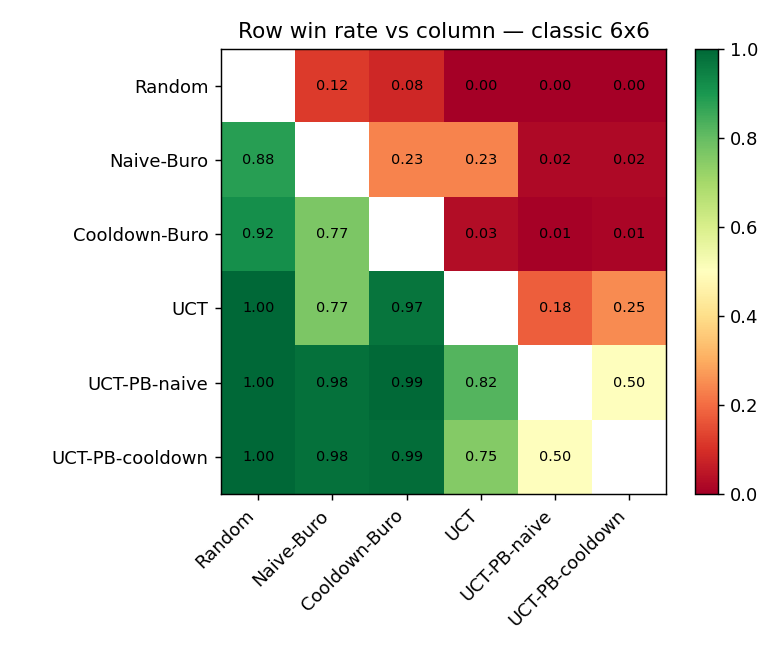
\includegraphics[width=\linewidth]{../05-analysis/figures/heatmap_winrate_classic.png}
    \caption{Klasyczne 6$\times$6}
  \end{subfigure}\hfill
  \begin{subfigure}{0.49\textwidth}\centering
    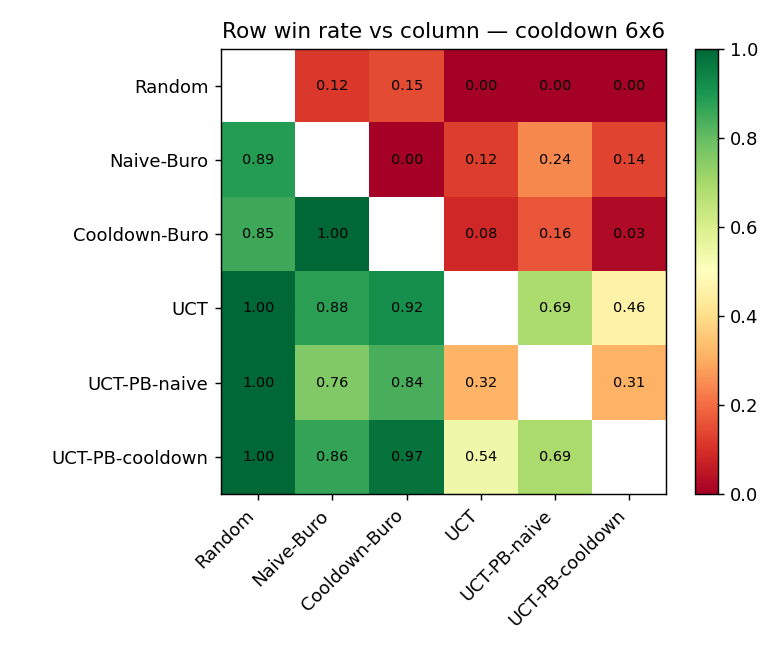
\includegraphics[width=\linewidth]{../05-analysis/figures/heatmap_winrate_cooldown.png}
    \caption{Cooldown 6$\times$6}
  \end{subfigure}
  \caption{Współczynnik wygranych gracza w~wierszu przeciw graczowi w~kolumnie.}
  \label{fig:heatmaps}
\end{figure}

\subsection{Różnice pionków i~metryki reguły}
Rysunek~\ref{fig:extra} (lewy) pokazuje rozkłady różnicy pionków na końcu partii, a~(prawy) metryki
specyficzne dla reguły: \emph{whipsaw rate} (jak często w~klasyku padłby ruch nielegalny pod regułą)
oraz \emph{cooldown-blocked rate} (jak często reguła blokuje atrakcyjny ruch).

\begin{figure}[H]\centering
  \begin{subfigure}{0.49\textwidth}\centering
    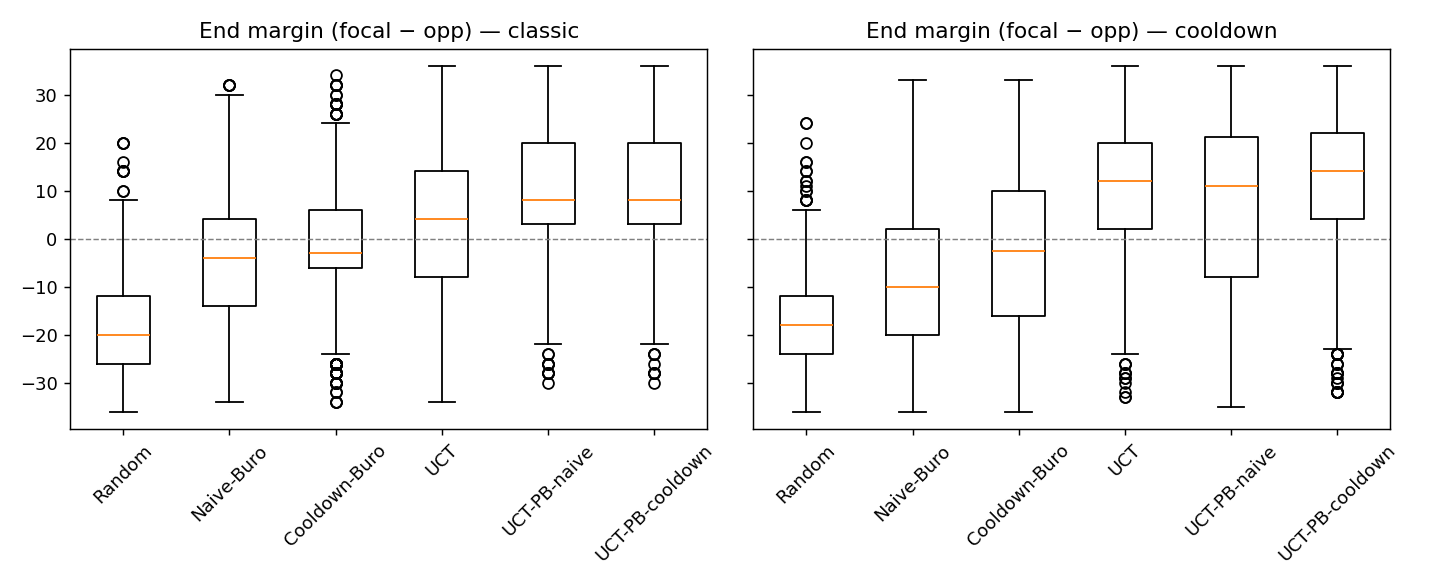
\includegraphics[width=\linewidth]{../05-analysis/figures/margin_boxplots.png}
    \caption{Różnica pionków (focal $-$ przeciwnik)}
  \end{subfigure}\hfill
  \begin{subfigure}{0.49\textwidth}\centering
    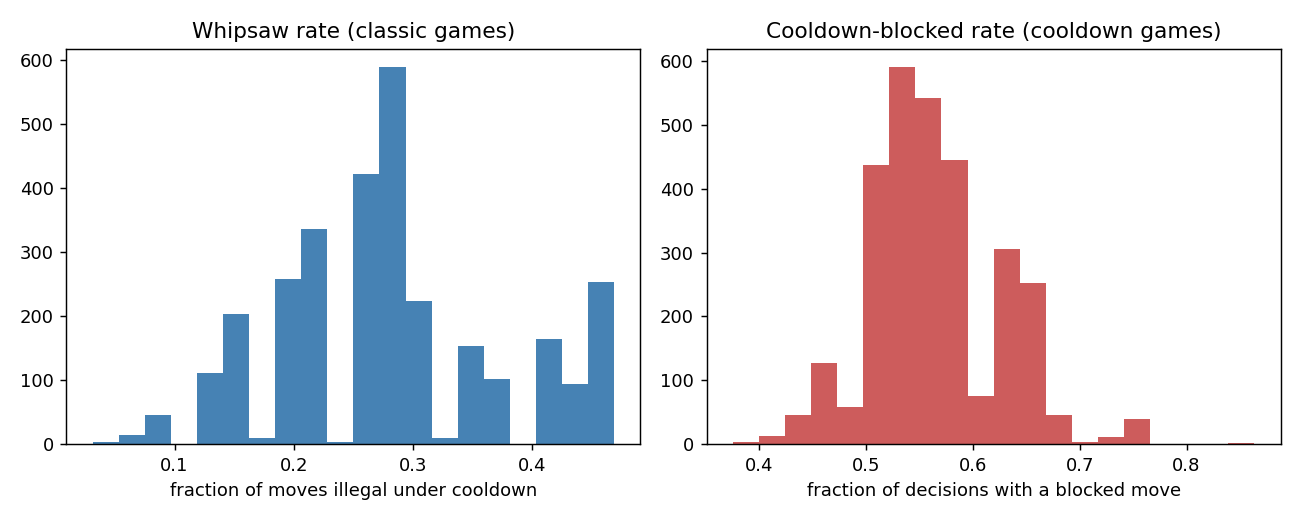
\includegraphics[width=\linewidth]{../05-analysis/figures/cooldown_metrics.png}
    \caption{Metryki reguły stygnięcia}
  \end{subfigure}
  \caption{Rozkłady wyników i~metryki specyficzne dla reguły.}
  \label{fig:extra}
\end{figure}

\subsection{Strojenie hiperparametrów}
Rysunek~\ref{fig:tuning} pokazuje zależność funkcji celu od stałej eksploracji $c$ dla UCT. Na
klasyku funkcja jest niemal płaska (UCT przytłacza zestaw kontrolny, więc $c$ jest słabo
ograniczone), na Cooldown widać łagodną preferencję małego $c$. To wyjaśnia, dlaczego strojone $c$
wypada po przeciwnych stronach zakresu dla obu wariantów.

\begin{figure}[H]\centering
  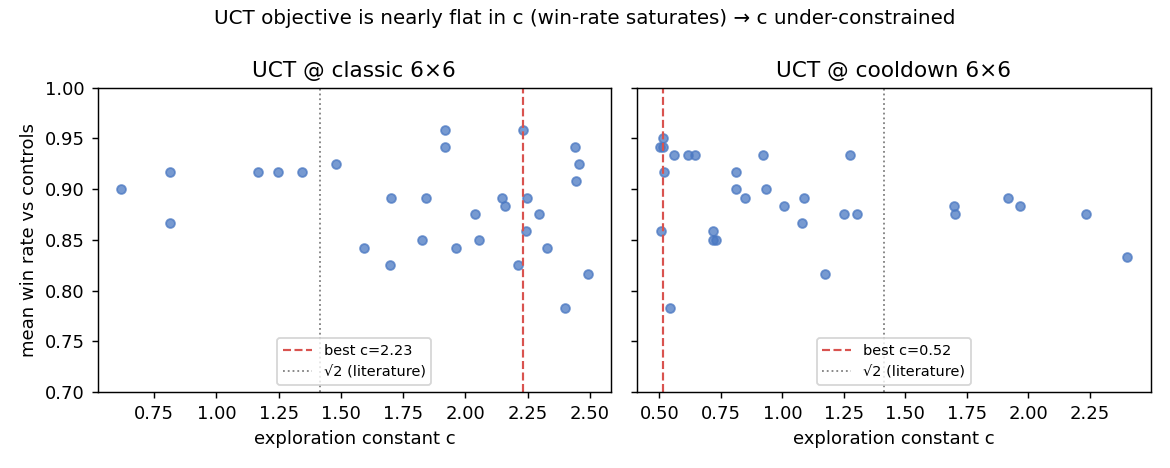
\includegraphics[width=0.9\textwidth]{../05-analysis/figures/tuning_uct_c_sensitivity.png}
  \caption{Zależność współczynnika wygranych UCT od stałej eksploracji $c$ (PDP/slice).}
  \label{fig:tuning}
\end{figure}

% ============================================================ 7. WERYFIKACJA HIPOTEZ
\section{Weryfikacja hipotez}
\begin{table}[H]
\centering
\small
\begin{tabular}{lrrrr}
\toprule
Hipoteza & Wynik & kluczowy efekt & $p$ & holm-$p$ \\
\midrule
H1 & potwierdzona & UCT vs Naive-Buro: 0.88 cooldown / 0.77 klasyk & 0.000 & 0.000 \\
H2 & odrzucona & przewaga UCT-PB-cooldown nad UCT: 4 p.p. & 0.289 & 0.289 \\
H3 & odrzucona & Cooldown-Buro vs Naive-Buro: 50 p.p. cooldown / 26 p.p. klasyk & 0.000 & 0.000 \\
H4 & potwierdzona & biały (2.~gracz): 0.58 klasyk / 0.49 cooldown & 0.000 & 0.000 \\
\bottomrule
\end{tabular}
\caption{Weryfikacja hipotez (wielkość efektu, $p$-wartość testu i~$p$ po korekcie Holma--Bonferroniego).}
\label{tab:hypotheses}
\end{table}

\paragraph{H1 -- potwierdzona.} UCT pokonuje Naive-Buro w~88\% na Cooldown (95\% CI: 0,82--0,92;
$\geq$60\%) i~w~77\% na klasyku; przewaga jest o~ok.\ 11~p.p.\ większa pod regułą stygnięcia
($p\!\approx\!10^{-29}$). Zgodnie z~intuicją -- reguła komplikuje ocenę pozycyjną, a~MCTS lepiej
radzi sobie z~zależnością od historii.

\paragraph{H2 -- odrzucona.} UCT-PB-cooldown pokonuje bazowy UCT na Cooldown jedynie o~ok.\ 4~p.p.\
(próg 10~p.p.\ nieosiągnięty, różnica nieistotna). Co więcej, UCT-PB-naive \emph{przegrywa}
z~bazowym UCT. Wniosek: progressive bias pomaga tylko z~heurystyką świadomą reguły i~to nieznacznie,
a~z~heurystyką naiwną szkodzi.

\paragraph{H3 -- odrzucona.} Na Cooldown Cooldown-Buro pokonuje Naive-Buro w~100\% (przewaga
$\gg$10~p.p.), ale na klasyku również wygrywa (o~ok.\ 26~p.p.), zamiast być równoważna. Heurystyka
świadoma reguły jest więc po prostu lepsza w~obu wariantach -- jej człon ,,trwałości bicia'' jest
użyteczny także w~klasycznym Othello -- więc nie udało się wyizolować efektu samej reguły.

\paragraph{H4 -- potwierdzona.} W~samogrze najsilniejszego wariantu (po 2000~partii na wariant)
drugi gracz (biały) wygrywa 58,4\% partii na klasycznym 6$\times$6 (95\% CI: 0,562--0,605; istotnie
$>$50\%), ale tylko 49,1\% pod regułą stygnięcia (95\% CI: 0,469--0,513; nieodróżnialne od~50\%).
Strukturalna przewaga drugiego gracza istnieje więc w~klasyku i~\emph{zanika} pod regułą stygnięcia
-- zgodnie z~intuicją, że eliminacja whipsaw odbiera graczowi odpowiadającemu reaktywną przewagę.

% ============================================================ 8. PODSUMOWANIE
\section{Podsumowanie i~wnioski}
Spośród czterech hipotez potwierdziły się dwie (H1, H4), a~dwie odrzuciliśmy (H2, H3) -- przy czym
odrzucenia są pouczające, nie negatywne.
Najsilniejszym graczem okazał się UCT-PB-cooldown, choć jego przewaga nad bazowym UCT jest
niewielka -- główny zysk pochodzi z~samego MCTS, nie z~progressive bias. Reguła stygnięcia realnie
zmienia grę (obniża rozgałęzienie, karze ,,naiwne'' bicia), co najmocniej widać w~zapaści
Naive-Buro na Cooldown. Zaskakującym wynikiem jest to, że heurystyka świadoma reguły pomaga także
w~klasycznym Othello -- sugeruje to, że ,,trwałość bicia'' jest ogólnie wartościowym sygnałem, a~nie
tylko sztuczką pod jedną regułę. Reguła zmienia też balans gry: znika strukturalna przewaga
drugiego gracza, co czyni Cooldown Othello bardziej zrównoważonym wariantem.

Ograniczeniem badania jest słaba czułość funkcji celu strojenia dla silnych graczy (płaska
zależność od~$c$), przez co część hiperparametrów MCTS jest słabo ograniczona; w~dalszych pracach
warto wzmocnić zestawy kontrolne. Eksperyment człowiek--komputer pozostawiamy jako naturalne
rozszerzenie (gotowy interfejs webowy).

% ============================================================ 9. LLM
\section{Wykorzystanie dużych modeli językowych}
Projekt zrealizowano z~użyciem asystenta opartego o~duży model językowy (Claude, Anthropic) w~roli
pary programistycznej: implementacja silnika gry i~wariantów MCTS, skryptów strojenia i~analizy,
orkiestracja eksperymentów na maszynie zdalnej oraz redakcja niniejszego raportu. Wszystkie decyzje
projektowe, weryfikacja poprawności (testy jednostkowe i~różnicowe) oraz interpretacja wyników były
nadzorowane przez autora.

% ============================================================ BIBLIOGRAFIA
\bibliography{references}

\end{document}
